% Paquets généraux
\documentclass[a4paper,12pt,titlepage]{article}
\usepackage[T1]{fontenc}
\usepackage[utf8]{inputenc}
\usepackage[french]{babel}
\usepackage[gen]{eurosym}
%\usepackage[dvips]{graphicx}
\usepackage{fancyhdr}
\usepackage{pdfpages} 
\usepackage{multido}
\usepackage{hyperref}
%\usepackage{textcomp}
%\usepackage{aeguill}
\usepackage{schemabloc}
\usepackage[bitstream-charter]{mathdesign}
\usepackage{minted}

\newcommand{\id}{71}
\newcommand{\nom}{Théorie des mécanismes}
\newcommand{\sequence}{04}
\newcommand{\nomsequence}{Liaisons entre les solides}
\newcommand{\num}{02}
\newcommand{\type}{KH}
\newcommand{\descrip}{Liaisons équivalentes, hyperstatisme, liaisons en série et en parallèle, théorie des graphes}
\newcommand{\competences}{B2-12: Proposer une modélisation des liaisons avec leurs caractéristiques géométriques. \\ &  B2-13: Proposer un modèle cinématique paramétré à partir d'un système réel, d'une maquette numérique ou d'u \\ &  B2-17: Simplifier un modèle de mécanisme. \\ &  B2-18: Modifier un modèle pour le rendre isostatique. \\ &  C1-04: Proposer une démarche permettant d'obtenir une loi entrée-sortie géométrique.  \\ &  C2-05: Caractériser le mouvement d'un repère par rapport à un autre repère. \\ &  C2-06: Déterminer les relations entre les grandeurs géométriques ou cinématiques. }
\newcommand{\nbcomp}{7}
\newcommand{\systemes}{}
\newcommand{\systemesnum}{}
\newcommand{\systemessansaccent}{}
\newcommand{\ilot}{2}
\newcommand{\ilotstr}{02}
\newcommand{\dossierilot}{\detokenize{Ilot_02 }}


\newcommand{\auteurun}{Renaud Costadoat}
\newcommand{\auteurdeux}{Françoise Puig}
\newcommand{\institute}{Lycée Dorian}


\usepackage{color}
\usepackage{xcolor}
\usepackage{colortbl}
\usepackage{helvet}
\usepackage[frenchmath]{newtxsf} % for sans serif symbols
\renewcommand{\familydefault}{\sfdefault}
%\usepackage{amsfonts}
%\usepackage{amsmath}
%\usepackage{lmodern}
\usepackage{mathastext}
%\usepackage{xspace}
\usepackage{varioref}
\usepackage{tabularx}
%\usepackage{floatflt}
\usepackage{graphics}
\usepackage{wrapfig}
\usepackage{textcomp}
\usepackage{tikz}
\usepackage{wrapfig}
\usepackage{gensymb}
\usepackage[european]{circuitikz}
\usetikzlibrary{babel}
\usepackage{ifthen}
\usepackage{cancel}
\usepackage{etoolbox}
\usepackage{multirow}
%\usepackage{boxedminipage}
\definecolor{gris25}{gray}{0.75}
\definecolor{bleu}{RGB}{18,33,98}
\definecolor{bleuf}{RGB}{42,94,171}
\definecolor{bleuc}{RGB}{231,239,247}
\definecolor{rougef}{RGB}{185,18,27}
\definecolor{rougec}{RGB}{255,188,204}%255,230,231
\definecolor{vertf}{RGB}{103,126,82}
\definecolor{vertc}{RGB}{220,255,191}
\definecolor{forestgreen}{rgb}{0.13,0.54,0.13}
\definecolor{blcr}{rgb}{0.59,0.69,0.84}
\definecolor{blfr}{rgb}{0.32,0.51,0.75}
\definecolor{orfr}{rgb}{0.90,0.42,0.15}
\definecolor{orcr}{rgb}{0.90,0.65,0.50}
\definecolor{orangef}{rgb}{0.659,0.269,0.072}
\definecolor{orange}{rgb}{0.58,0.35,0.063}
\definecolor{orangec}{rgb}{0.43,0.32,0.25}
\definecolor{rcorrect}{rgb}{0.6,0,0}
\definecolor{sequence}{rgb}{0.75,0.75,0.75}
\definecolor{competences}{rgb}{0.61,0.73,0.35}
\definecolor{grisf}{HTML}{222222}
\definecolor{grisc}{HTML}{636363}
\definecolor{normal}{HTML}{4087c4}
\definecolor{info}{HTML}{5bc0de}
\definecolor{success}{RGB}{92,184,92}
\definecolor{warning}{RGB}{240,173,78}
\definecolor{danger}{RGB}{217,83,79}
\hypersetup{                    % parametrage des hyperliens
    colorlinks=true,                % colorise les liens
    breaklinks=true,                % permet les retours à la ligne pour les liens trop longs
    urlcolor= blfr,                 % couleur des hyperliens
    linkcolor= orange,                % couleur des liens internes aux documents (index, figures, tableaux, equations,...)
    citecolor= forestgreen                % couleur des liens vers les references bibliographiques
    }

% Mise en page
\pagestyle{fancy}

\setlength{\hoffset}{-18pt}

\setlength{\oddsidemargin}{0pt} 	% Marge gauche sur pages impaires
\setlength{\evensidemargin}{0pt} 	% Marge gauche sur pages paires
\setlength{\marginparwidth}{00pt} 	% Largeur de note dans la marge
\setlength{\headwidth}{481pt} 	 	% Largeur de la zone de tête (17cm)
\setlength{\textwidth}{481pt} 	 	% Largeur de la zone de texte (17cm)
\setlength{\voffset}{-18pt} 		% Bon pour DOS
\setlength{\marginparsep}{7pt}	 	% Séparation de la marge
\setlength{\topmargin}{-30pt} 		% Pas de marge en haut
\setlength{\headheight}{35pt} 		% Haut de page
\setlength{\headsep}{20pt} 		% Entre le haut de page et le texte
\setlength{\footskip}{30pt} 		% Bas de page + séparation
\setlength{\textheight}{700pt} 		% Hauteur de l'icone zone de texte (25cm)
\setlength\fboxrule{1 pt}
\renewcommand{\baselinestretch}{1}
\setcounter{tocdepth}{1}
\newcommand{\cadre}[2]
{\fbox{
  \begin{minipage}{#1\linewidth}
   \begin{center}
    #2\\
   \end{center}
  \end{minipage}
 }
}

\newcounter{num_quest} \setcounter{num_quest}{0}
\newcounter{num_rep} \setcounter{num_rep}{0}
\newcounter{num_cor} \setcounter{num_cor}{0}

\newcommand{\question}[1]{\refstepcounter{num_quest}\par
~\ \\ \parbox[t][][t]{0.15\linewidth}{\textbf{Question \arabic{num_quest}}}\parbox[t][][t]{0.93\linewidth}{#1}\par
}


\newcommand{\reponse}[1]
{\refstepcounter{num_rep}
\noindent
\rule{\linewidth}{.5pt}
\textbf{Question \arabic{num_rep}:}
\multido{\i=1+1}{#1}{~\ \\}
}

\newcommand{\cor}
{\refstepcounter{num_cor}
\noindent
\rule{\linewidth}{.5pt}
\textbf{Question \arabic{num_cor}:} \\
}

\newcommand{\titre}[1]
{\begin{center}
\cadre{0.8}{\huge #1} 
\end{center}
}


% En tête et pied de page
\fancypagestyle{normal}{%
  \fancyhf{}
\lhead{\nom}
\rhead{
\includegraphics[width=2cm]{../../img/logo}\hspace{2pt}}
\ifdef{\auteurdeux}{\lfoot{\auteurun,\auteurdeux}}{\lfoot{\auteurun}}
\cfoot{Page \thepage}}

\fancypagestyle{correction}{%
  \fancyhf{}
  \lhead{\colorbox{danger}{\begin{minipage}{0.65\paperwidth} \textcolor{white}{\textbf{Correction}} \end{minipage}} }
  \rhead{
\includegraphics[width=2cm]{../../img/logo}}
  \ifdef{\auteurdeux}{\lfoot{\auteurun,\auteurdeux}}{\lfoot{\auteurun}}
  \rfoot{\colorbox{danger}{\begin{minipage}{0.5\paperwidth} \begin{flushright}\textcolor{white}{\textbf{Correction}}\end{flushright} \end{minipage}} }}

\renewcommand{\footrulewidth}{0.4pt}

\usepackage{eso-pic}
\newcommand{\BackgroundPic}{%
\put(0,0){%
\parbox[b][\paperheight]{\paperwidth}{%
\vfill
\begin{center}
\hspace{0.5cm}\vspace{0.5cm}
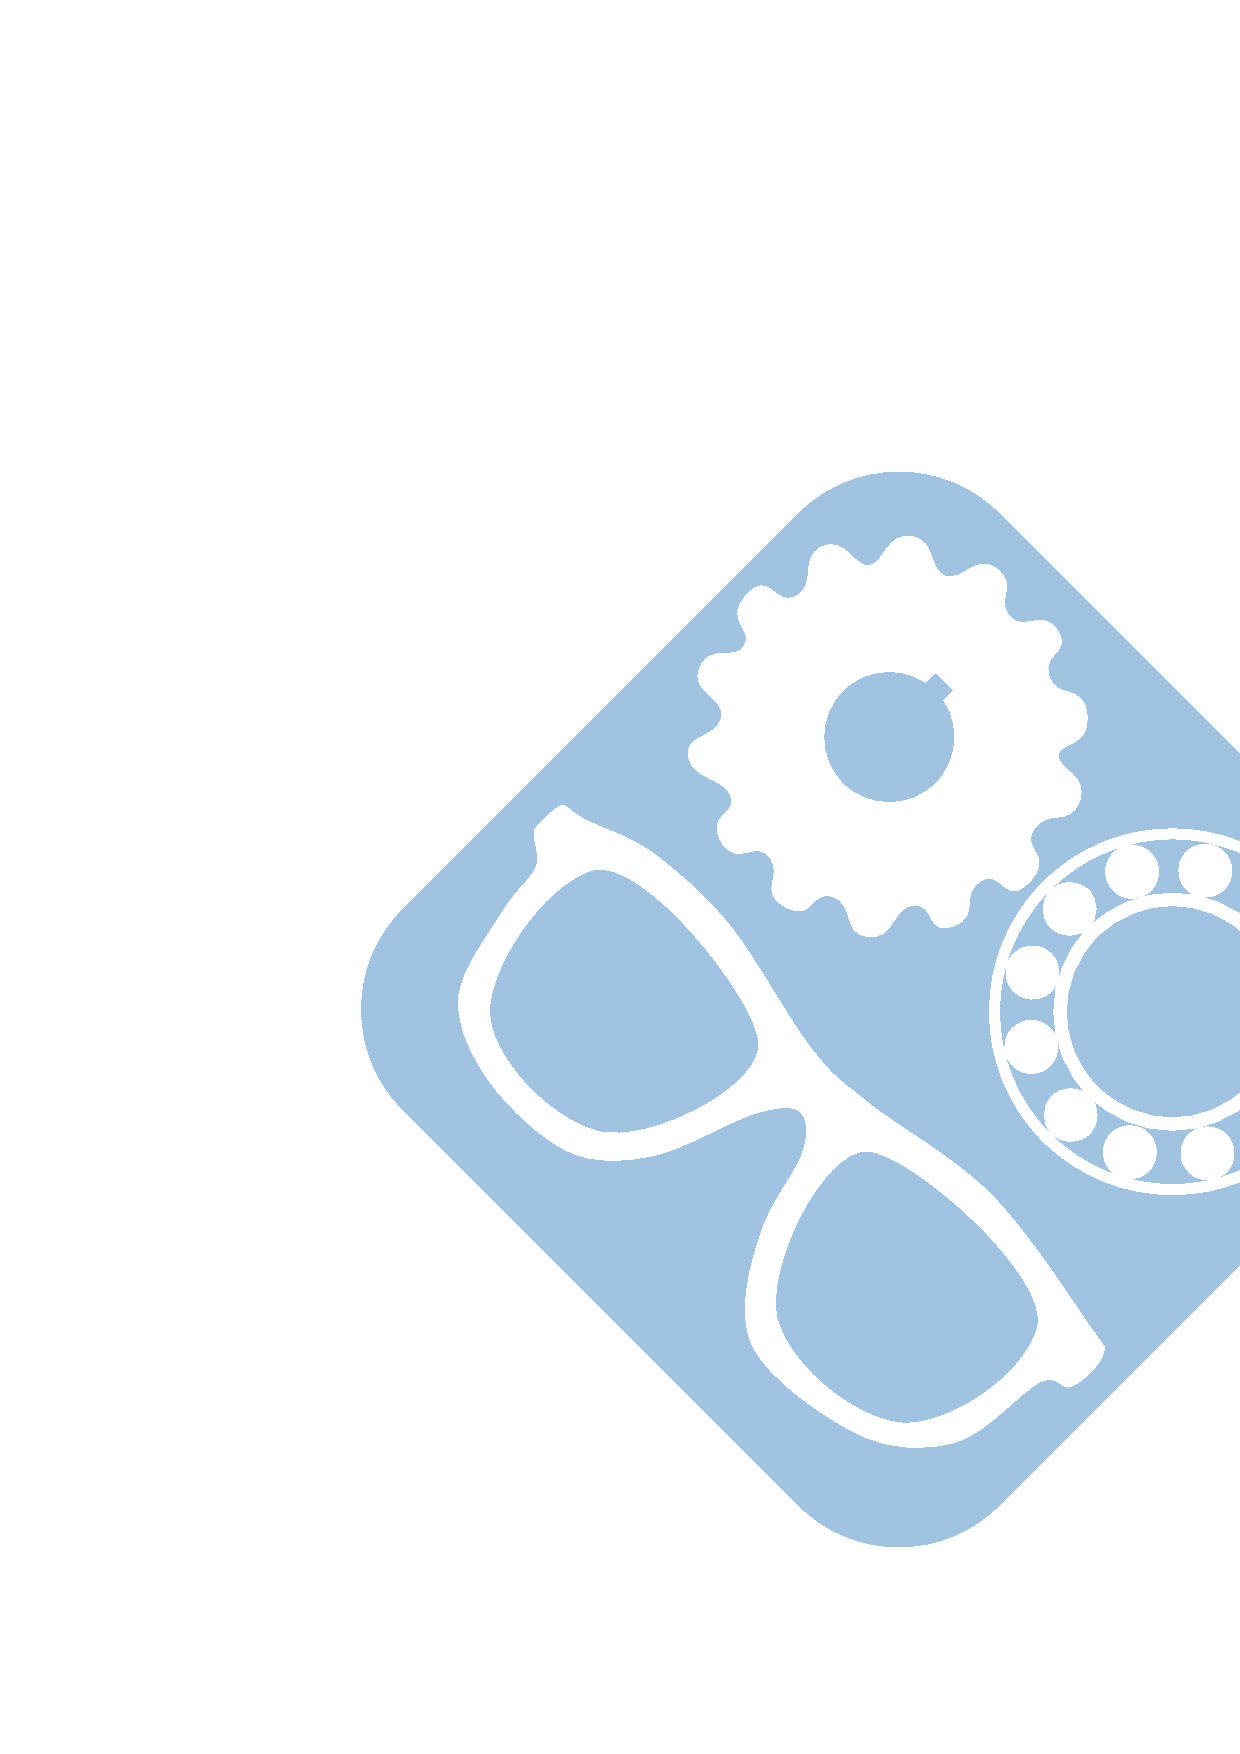
\includegraphics[width=\paperwidth,height=\paperheight,%
keepaspectratio]{../../img/fond3}%
\end{center}
\vfill
}}}

\newcommand{\BackgroundPicdeux}{%
\put(25,-30){%
\parbox[b][\paperheight]{\paperwidth}{%
\vfill
\begin{center}
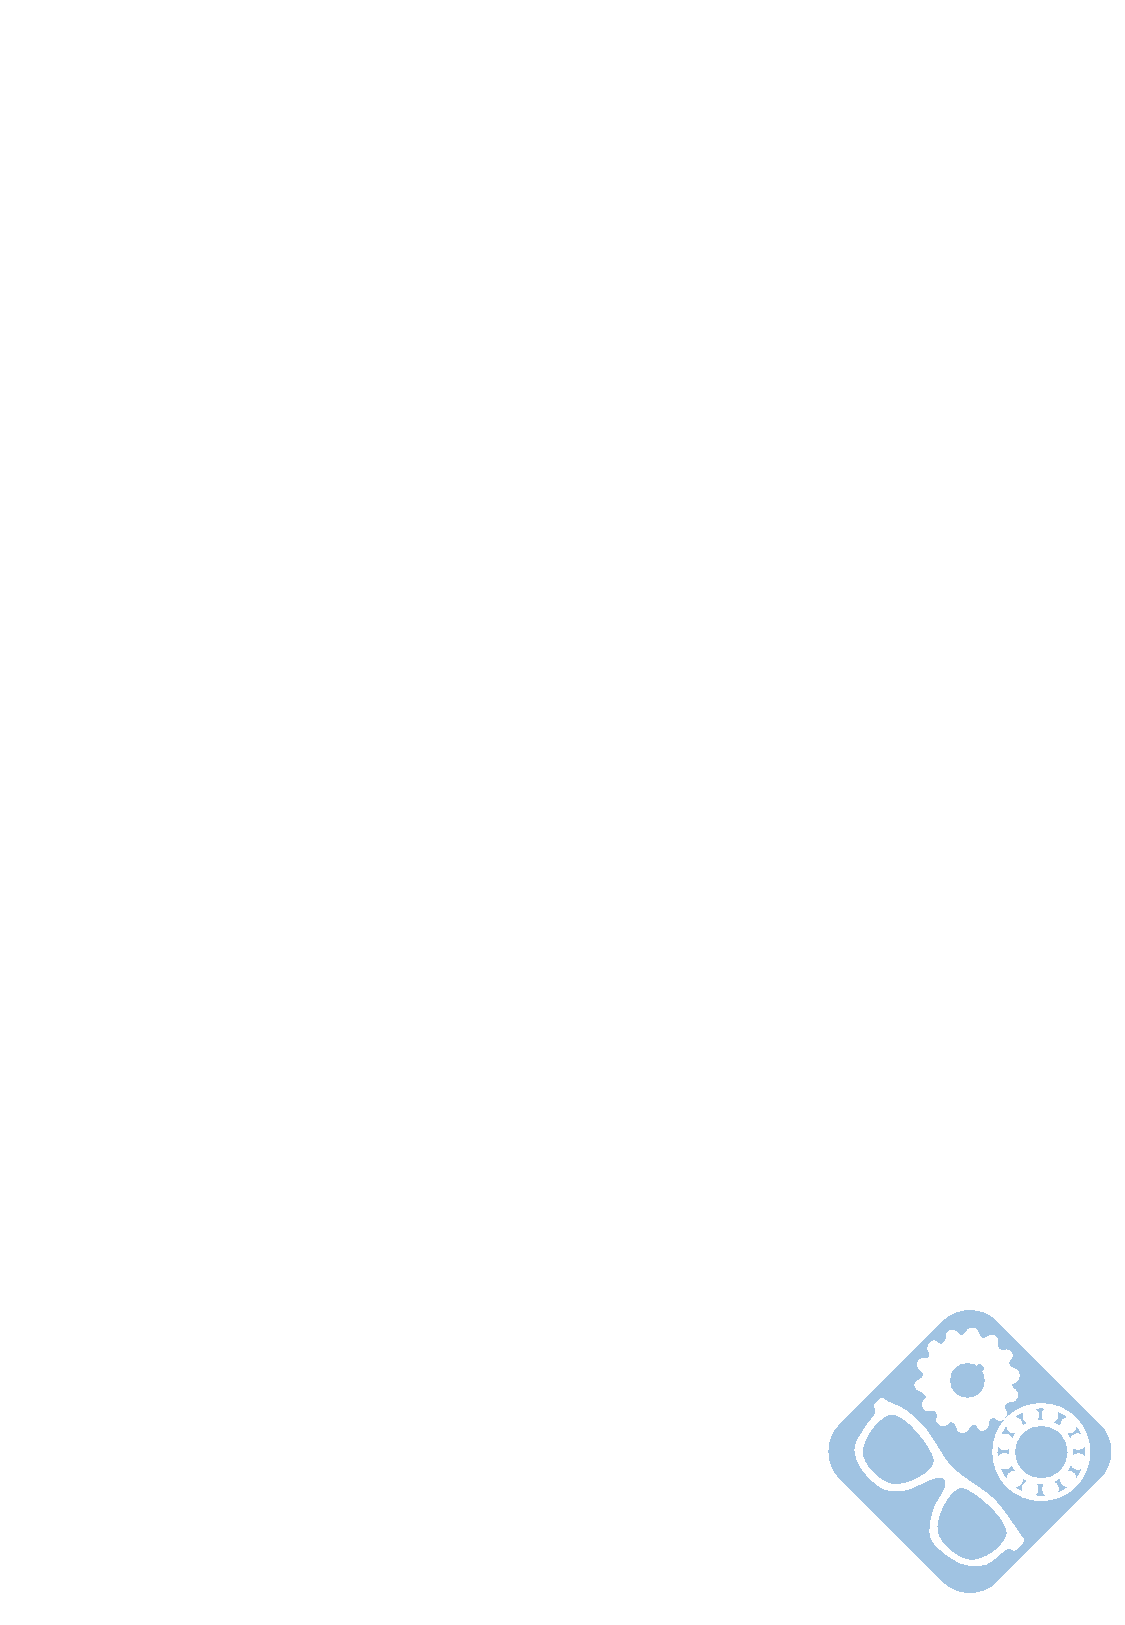
\includegraphics[width=\paperwidth,height=\paperheight,%
keepaspectratio]{../../img/fond4}%
\end{center}
\vfill
}}}

\begin{document}

\pagestyle{empty}

\vspace*{-3\baselineskip}

\AddToShipoutPicture*{\BackgroundPic}

\ifdef{\auteurdeux}{\begin{tabular}{>{\columncolor{gray!00}}m{.3\linewidth} m{.3\linewidth} >{\columncolor{gray!00}}m{.3\linewidth}}
Séquence : \sequence &  \multirow{3}{*}{\hspace{1cm}
\includegraphics[height=1.5cm]{../../img/logo}} &  \begin{flushright} \multirow{4}{*}{\hspace{1cm}\includegraphics[height=4cm]{img/qrcode}}\end{flushright}\\
Document : \type\num \\
 \institute \\
 \auteurun\\
 \auteurdeux
\end{tabular}}{\begin{tabular}{>{\columncolor{gray!00}}m{.3\linewidth} m{.3\linewidth} >{\columncolor{gray!00}}m{.3\linewidth}}
Séquence : \sequence &  \multirow{3}{*}{\hspace{1cm}
\includegraphics[height=1.5cm]{../../img/logo}} &  \begin{flushright} \multirow{4}{*}{\hspace{1cm}\includegraphics[height=4cm]{img/qrcode}}\end{flushright}\\
Document : \type\num \\
 \institute \\
 \auteurun
\end{tabular}}

\vspace{1cm}

\ifdef{\prive}{\begin{center}\colorbox{danger}{\Huge{Avec Correction}}\end{center}}{}

\begin{center}\huge{\nom}\end{center}

\vspace{2cm}

\ifdef{\imagedeux}{\begin{minipage}{0.49\linewidth}}{}
\begin{center}\includegraphics[height=5cm]{/home/renaud/Documents/Renaud/GitHub/django_education/systemes/\imageun}\end{center}
\ifdef{\imagedeux}{\end{minipage}\hfill
\begin{minipage}{0.49\linewidth}
\begin{center}\includegraphics[height=5cm]{/home/renaud/Documents/Renaud/GitHub/django_education/systemes/\imagedeux}\end{center}
\end{minipage}}{}

\vspace{5cm}


\begin{tabular}{p{.15\linewidth} >{\columncolor{white}}p{.8\linewidth}}
    \rowcolor{gray!20}
    Référence & S\sequence\ - \type\num \\
    Compétences & \competences \\
 	\rowcolor{gray!20}
    Description & \descrip \\
    Système & \systemes
  \end{tabular}

\newpage

\AddToShipoutPicture{\BackgroundPicdeux}

\pagestyle{normal}

\section{Couple de freinage}

Les disques de freinage sont utilisés sur les véhicules automobiles mais aussi sur certains vélos qui ont besoin de hautes performances. Le fonctionnement consiste à presser sur un disque métallique une ou plusieurs plaquettes et de dissiper l'énergie cinétique par des frottements.

\begin{minipage}{0.47\linewidth}
 \centering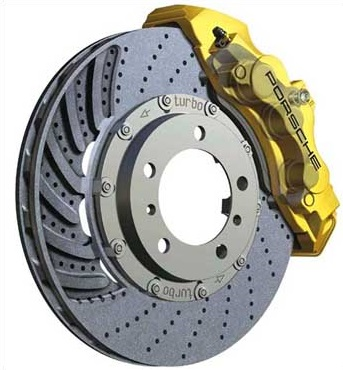
\includegraphics[width=0.5\linewidth]{img/disque}
\end{minipage}\hfill
\begin{minipage}{0.47\linewidth}
 \centering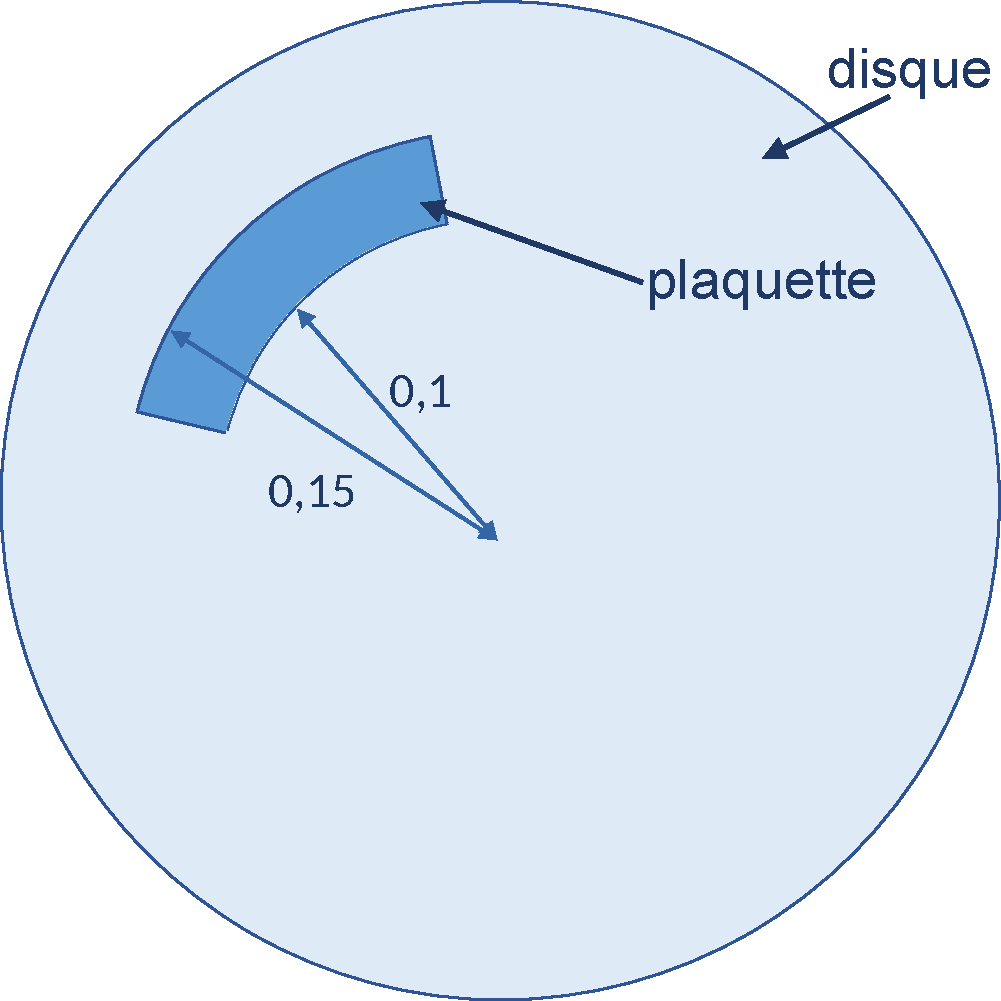
\includegraphics[width=0.5\linewidth]{img/Frein_1}
\end{minipage}

~\

Le cas suivant présente un disque en contact avec une plaquette dont les caractéristiques sont les suivantes:
\begin{itemize}
 \item Rayon intérieur : $R_{int}=10cm$,
 \item Rayon extérieur : $R_{ext}=15cm$,
 \item Angle de la plaquette : $\theta=\dfrac{\pi}{2}\ \mathrm{rad}$,
 \item Le coefficient de frottement avec le disque est $f=0,3$.
\end{itemize}

~\

La liaison ne peut pas être modélisée par une liaison appui plan car l'effort du contact n'est pas homogène sur toute la surface. C'est pour cela que nous allons considérer que la liaison est constituée d'une infinité de contacts ponctuels. La liaison équivalente appui plan sera obtenue en ajoutant les torseurs des liaisons ponctuelles, celles-ci étant en parallèle.

~\

\begin{minipage}{0.47\linewidth}
Afin d'effectuer une étude numérique, nous découpons la surface de contact en plusieurs surfaces $dS$ afin d'effectuer un calcul infinitésimal. L'angle $\theta$ sera décomposé en $Nt$ angles $d\theta$ et la distance $(R_{ext}-R_{int})$ sera décomposée en $Nr$ distances $dr$.

\paragraph{Question 1:} Écrire $dr$ en fonction de $R_{ext}$, $R_{int}$ et $Nr$. Écrire $d\theta$ en fonction de $\theta$ et $Nt$.
\end{minipage}\hfill
\begin{minipage}{0.47\linewidth}
 \centering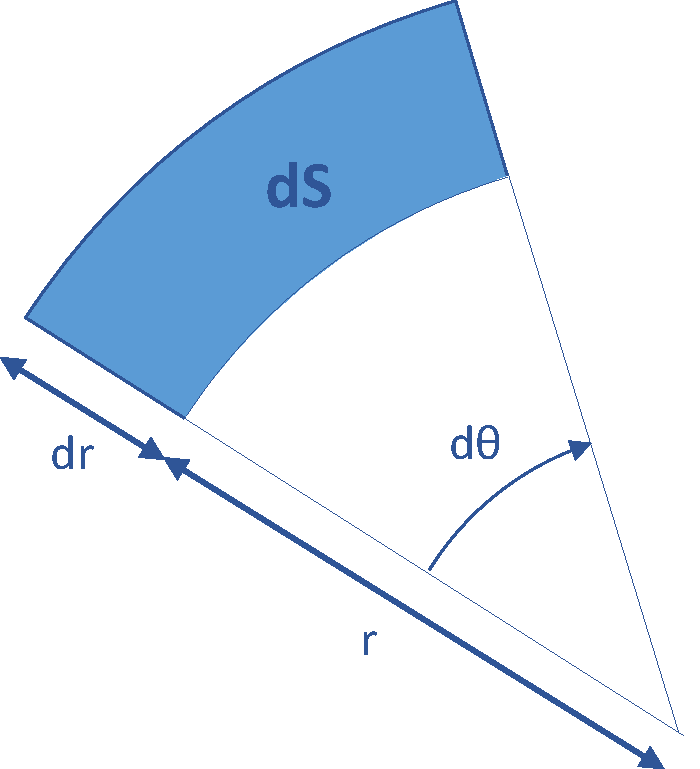
\includegraphics[width=0.6\linewidth]{img/Frein_2}
\end{minipage}

~\

\begin{minipage}{0.47\linewidth}
 \centering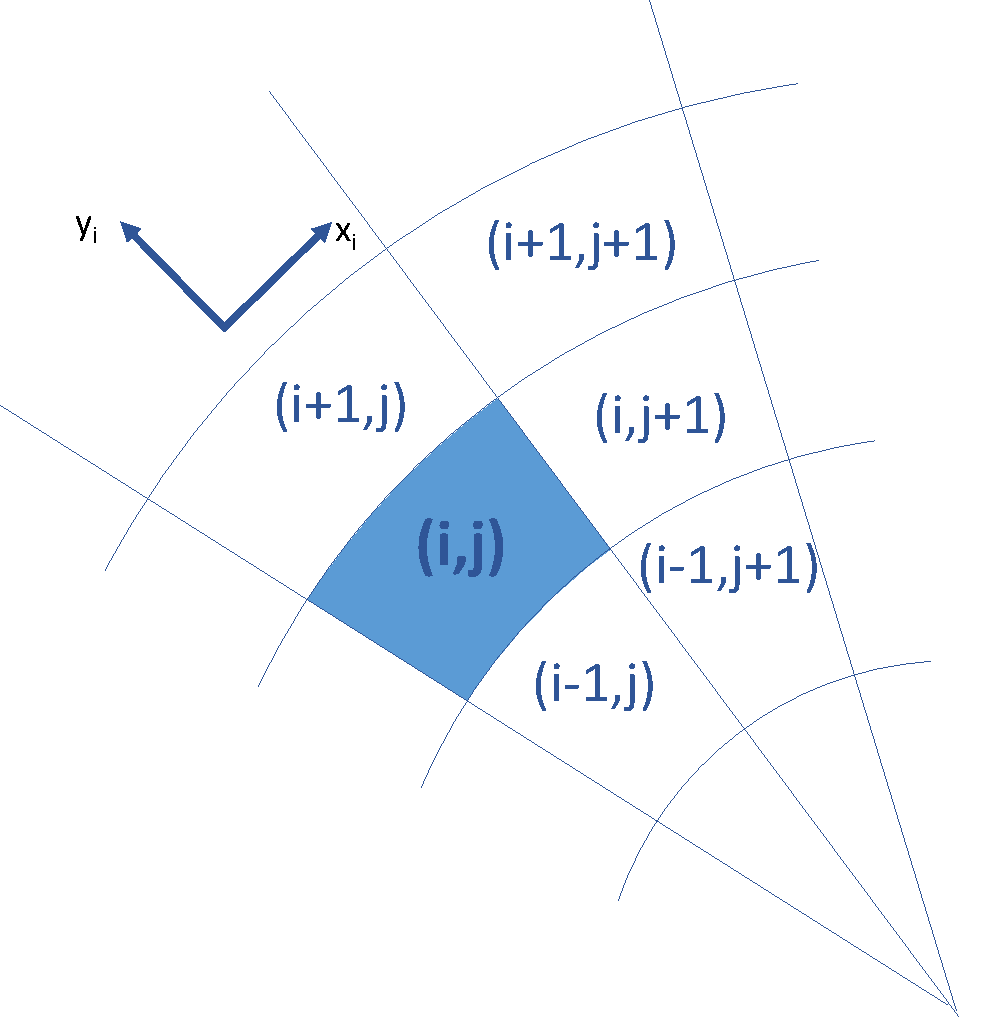
\includegraphics[width=0.7\linewidth]{img/Frein_3}
\end{minipage}\hfill
\begin{minipage}{0.47\linewidth}
Afin de parcourir, l'ensemble de $Nt\times Nr$ surfaces $dS$ ainsi créées, nous allons donner à chacune d'entre elles des coordonnées $(i,j)$, comme le montre la figure ci-contre. ($i$ et $j$ démarrent à $0$).

\paragraph{Question 2:} Écrire $dS$ en fonction de $R_{int}$, $i$, $dr$ et $d\theta$.
\end{minipage}

Le coefficient $f=\dfrac{p}{q}$ permet de modéliser les frottement entre le disque et une plaquette. Il permet de lier l'effort normal et l'effort tangentiel qui s'appliquent entre les deux pièces. La force élémentaire normale exercée sur la surface $(i,j)$ peut alors s'écrire $dF_n=P.dS$, avec $P$ la pression exercée entre le disque et la plaquette. L'effort tangentiel s'écrit alors $dF_t=f.P.dS$.

Soit $M$ le centre de la surface $(i,j)$, le torseur en un point M d'une liaison ponctuelle, avec frottement, entre le disque et la plaquette s'écrit s'écrit :

$\left\{T_{D\rightarrow P}\right\}=\left\{\begin{array}{c c}
dF_t & 0 \\ 0 & 0 \\ dF_n & 0
\end{array}\right\}_{M(\overrightarrow{x_j},\overrightarrow{y_j},\overrightarrow{z})}$

\paragraph{Question 3:} Soit $O$ le centre du disque, écrire le vecteur $\overrightarrow{OM}$ en fonction de $R_{int}$, $i$ et $dr$. En déduire le moment de force projeté autour de $\overrightarrow{z}$, lorsque l'action $dF_t$ est ramenée au point O: $(\overrightarrow{OM}\wedge \overrightarrow{dF_t}).\overrightarrow{z}$.

~\

Le couple de freinage est généré par l'ensemble de ces surfaces élémentaires $dS$, il faut donc intégrer ces moments sur toute la surface de contact.

~\

Remarque: Attention, il y a une plaquette de frein de chaque côté du disque.

Dans un premier temps, la pression sera considérée constante sur toute la surface du disque : $P_0=0,05Pa$. Faire le calcul pour $Nt=Nr=100$ et $Nt=Nr=1000$.

\paragraph{Question 4:} Déterminer le couple de freinage généré par ce frein à disque.

\paragraph{Question 5:} Un calcul littéral donne $Cf=2.\theta.f.P.\dfrac{R_{ext}^3-R_{int}^3}{3}$. Que constatez-vous compte tenu des résultats de la question 4 ?

~\

Dans la suite, la pression ne sera plus constante mais liée au rayon du point central de la surface par une formule de la forme : $P=a.r+b$, sachant que sur le rayon intérieur, la pression sera égale à 80\% de $P_0$ et sur le rayon extérieur 120\% de $P_0$.

\paragraph{Question 6:} Déterminer la pression $P$ en fonction de $r$ et en déduire le couple de freinage généré par ce frein à disque.

\section{La course du coureur}

Un coureur fait un exercice de course fractionné. C'est à dire qu'il va tenter de courir à une vitesse de :
\begin{enumerate}
 \item $9km\cdot h^{-1}$ pendant trois minutes,
 \item $14km\cdot h^{-1}$ pendant trois minutes,
 \item $9km\cdot h^{-1}$ pendant trois minutes,
 \item $14km\cdot h^{-1}$ pendant trois minutes,
 \item $9km\cdot h^{-1}$ pendant trois minutes,
 \item $14km\cdot h^{-1}$ pendant trois minutes.
\end{enumerate}

Le fichier \texttt{Course.txt} renvoie en première colonne le temps à partir du départ de la course et la deuxième colonne la vitesse.

Rappel : La fonction \verb? np.array=asarray(liste) ? de la bibliothèque Numpy permet de convertir une \verb? liste ? en \verb? array ?.

\paragraph{Question 1:} Tracer la vitesse du coureur en fonction du temps. 

\paragraph{Question 2:} Calculer le vecteur \verb? position ? qui définie la distance parcourue par le coureur à chaque instant. Déterminer la distance parcourue à la fin de l’entraînement.

\paragraph{Question 3:} Tracer le vecteur \verb? position ?. L'allure de la courbe vous paraît-elle cohérente ?

\ifdef{\public}{\end{document}}{}

\newpage

\pagestyle{correction}

\section{Correction}

\subsection{Couple de freinage}

\paragraph{Question 1:} $dr=\dfrac{R_{ext}-R_{int}}{Nr}$, $d\theta=\dfrac{\theta}{Nt}$

\paragraph{Question 2:} $ds=(R_{int}+dr*(i+\dfrac{1}{2}))*dr*d\theta$ 

\paragraph{Question 3:} $\overrightarrow{OM}=(R1+dr*(i+\dfrac{1}{2})).\overrightarrow{y_i}$

$(\overrightarrow{OM}\wedge \overrightarrow{dF_t}).\overrightarrow{z}=\left[(R1+dr*(i+\dfrac{1}{2})).\overrightarrow{y_i}\wedge dS.f.P.\overrightarrow{x_i}\right].\overrightarrow{z}=-(R1+dr*(i+\dfrac{1}{2})).dS.f.P$.

\paragraph{Question 4:} 

\begin{minted}[]{python}

theta=np.pi/2.
R2=0.15
R1=0.1
fr=0.3

Nt=1000
Nr=1000
dr=(R2-R1)/Nr
dt=theta/Nt

P0=0.05*10**6
C1=0

for i in range(Nr):
	for j in range(Nt):
		P=P0
		ds=(R1+dr*(i+1/2.))*dr*dt
		F=fr*ds*P
		C1=C1-2*F*(R1+dr*(i+1/2.))  
    
print(C1)

C2=-2*theta*fr*P*(R2**3-R1**3)/3.
print(C2)
\end{minted}



\paragraph{Question 5:} En augmentant $Nt$ et $Nr$, le résultat tend vers le calcul littéral. Ceci s'explique car la diminution du pas d'intégration améliore sa précision.

\paragraph{Question 6:} 

\begin{minted}[]{python}

theta=np.pi/2.
R2=0.15
R1=0.1
fr=0.3

Nt=1000
Nr=1000
dr=(R2-R1)/Nr
dt=theta/Nt

a=(0.4*P0)/(R2-R1)
b=0.8*P0-R1*a
C1=0

for i in range(Nr):
     for j in range(Nt):
         P=a*(R1+dr*(i+1/2.))+b
         ds=(R1+dr*(i+1/2.))*dr*dt
         F=fr*ds*P
         C1=C1-2*F*(R1+dr*(i+1/2.))  
    
print(C1)
\end{minted}

\subsection{La course du coureur}

\paragraph{Question 1, 2 et 3:}

\begin{minted}[]{python}

def lireFichier(fichier):
    lignes = [line for line in open(fichier,'r')]
    result=[]
    for element in lignes:
        temps,pace = map(float,element.split())
        result.append((temps,pace))
    return result

def convertms(v):
    return v/3.6

vitesse = np.asarray(lireFichier("Course.txt"))
plt.plot(vitesse[:,0],vitesse[:,1],"bo-")

pos=np.zeros(len(vitesse[:,0]))

for i in range(len(vitesse[:,0])-1):
    pos[i+1] = pos[i] + convertms(vitesse[i+1,1])*(vitesse[i+1,0]-vitesse[i,0])    
    
print(pos[len(vitesse[:,0])-1]/1000.)

plt.plot(vitesse[:,0],vitesse[:,1],"bo-")
plt.plot(vitesse[:,0],position,"r")
\end{minted}

\paragraph{Question 3:} L'allure de la courbe paraît cohérente car les différentes vitesses de course se retrouvent sur la pente de la position.

\end{document}
